\appendix

\section{Project directive and templates}
	
	\subsection{Contact information}
		\subsubsection{Customer}
			\begin{itemize}
				\item {\bf Askild Olsen} \newline
						Telephone: 73 59 21 93 \newline
						Mobile: 91 78 34 89 \newline
						Fax: 73 59 22 40 \newline
						E-mail: askild.olsen@artsdatabanken.no
				\item {\bf  Helge Sandmark} \newline
						E-mail: helge.sandmark@artsdatabanken.no
				\item {\bf Nils Valland} \newline
						Telephone: 73 59 23 01 \newline
						Mobile: 92 41 20 37 \newline
						Fax: 73 59 22 40 \newline
						E-mail: nils.valland@artsdatabanken.no
			\end{itemize}
			
		\subsubsection{Supervisor}
			\begin{itemize}
				\item {\bf Muhammad Asif} \newline
						Telephone: 73 59 36 71 \newline
						E-mail: muhamma@idi.ntnu.no
			\end{itemize}

		\subsubsection{Team members}
				\begin{itemize}
					\item {\bf Anders Søbstad Rye} \newline
							E-mail: anderrye@stud.ntnu.no
					\item {\bf Andreas Berg Skomedal} \newline
							E-mail: andrskom@stud.ntnu.no
					\item {\bf Dag-Inge Aas} \newline
							E-mail: dagingaa@stud.ntnu.no
					\item {\bf Muhsin Gnaydin} \newline
							E-mail: gunaydin@stud.ntnu.no
					\item {\bf Nikola Djoric} \newline
							E-mail: nikoladj@stud.ntnu.no
					\item {\bf Stian Liknes} \newline
							E-mail: stianlik@stud.ntnu.no
					\item {\bf Yonathan Redda} \newline
							E-mail: redda@stud.ntnu.no
				\end{itemize}
	\newpage
	\subsection{Meeting agendas}
		\begin{figure}[htb]
			\centering
			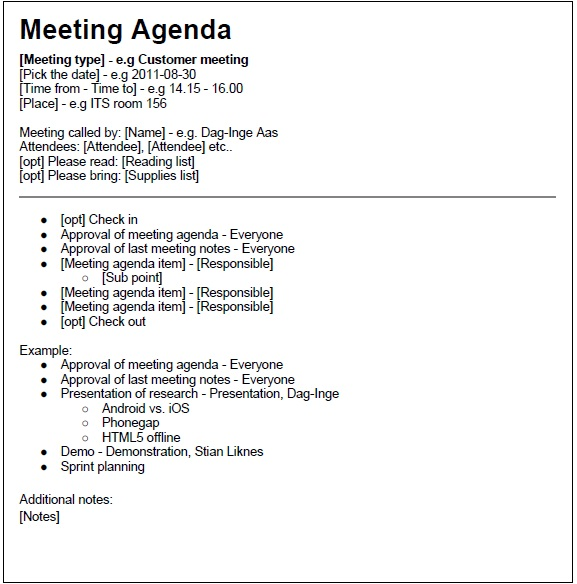
\includegraphics[width=0.8\textwidth]{appendix/meeting_agenda.jpg}
			\caption{Meeting agenda}
			\label{fig:meeting-agenda}
		\end{figure}
	
	\newpage
	\subsection{Meeting minutes}
		\begin{figure}[htb]
			\centering
			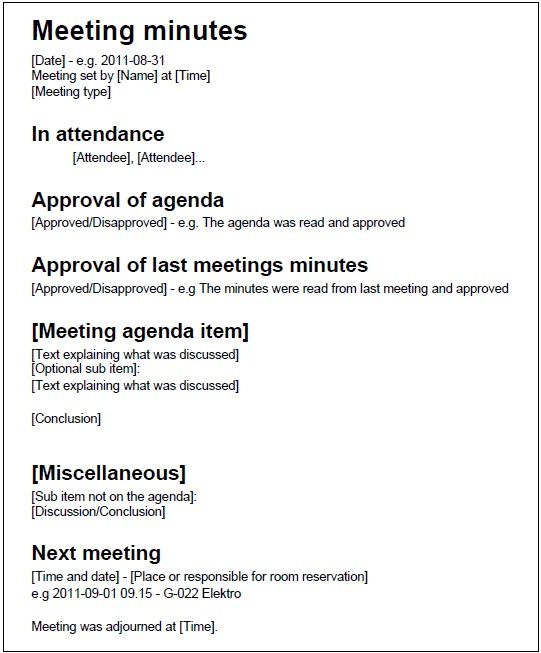
\includegraphics[width=0.8\textwidth]{appendix/meeting_minutes.jpg}
			\caption{Meeting minutes}
			\label{fig:meeting-minutes}
		\end{figure}
	
	\newpage
	\subsection{Weekly status report}
		\begin{figure}[htb]
			\centering
			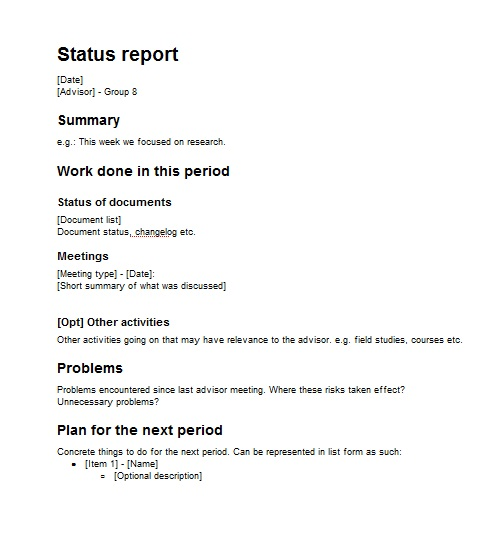
\includegraphics[width=0.8\textwidth]{appendix/weekly_status_report.jpg}
			\caption{Weekly status report}
			\label{fig:weekly-status-report}
		\end{figure}

\newpage
\section{User guide}
This portion of the document details installation guides for the user, in addition to a how-to for the application. This should provide the user with adequate information about how to install and use the application.
\subsection{Installation guide}
The application can be downloaded from the Android Market, with the name "Artsdatabanken". It can also be installed directly from an executable installation package, an apk, by going to the following url: \url{http://stuff.daginge.com/artsdatabanken.apk}.

\begin{figure}[h!]
\centering
 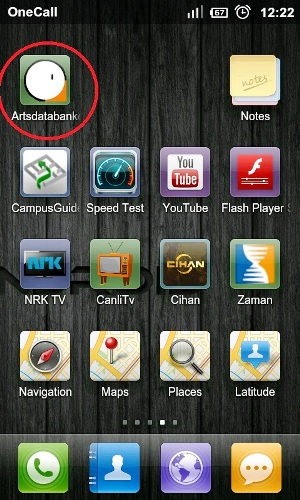
\includegraphics[width=0.6\textwidth,height=0.9\textwidth]{appendix/pic/run.jpg} 
 \caption{The program icon after installation}
 \end{figure}

\subsection{How-to}
\subsubsection{Creating an observation}
The user creates an observation by following the "Create an observation/Ny
Observasjon" link from the front page of the application.  From here, the user
selects which species group to observe.  This will lead the user to an
observation table, where the user can input species name, which is
auto-completed, and the number of individuals found.  Both common names and
scientific names are applicable. 

\begin{figure}[h!]
\centering
 \begin{center}$
 \begin{array}{cc}
 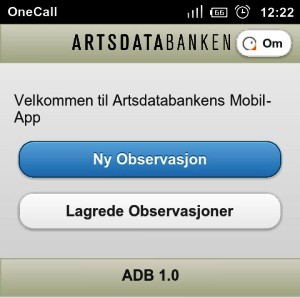
\includegraphics[width=0.6\textwidth,height=0.9\textwidth]{appendix/pic/nyobs.jpg} &
 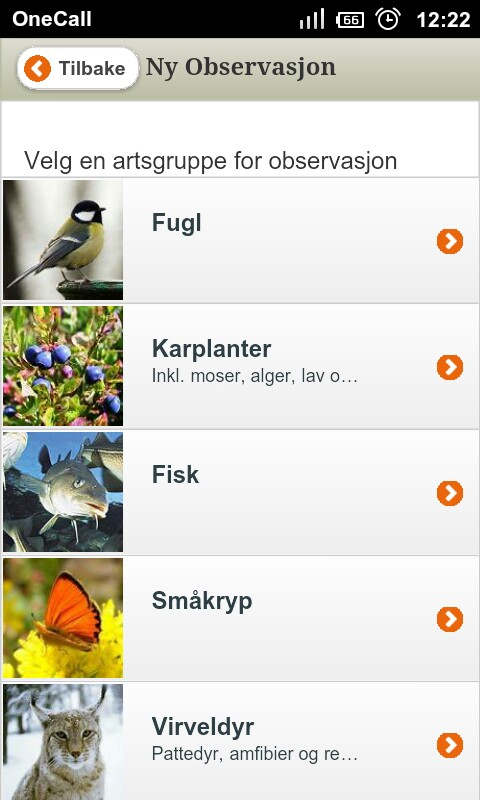
\includegraphics[width=0.6\textwidth,height=0.9\textwidth]{appendix/pic/velgart.jpg}
 \end{array}$
 \end{center}
 \caption{Front page (left). Select Species (right) }
 \end{figure}

\begin{figure}[h!]
\centering
 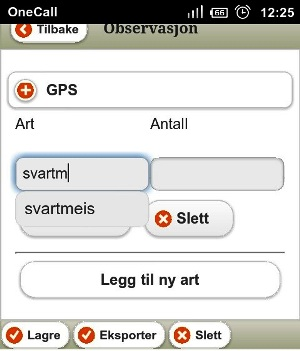
\includegraphics[height=0.6\textwidth]{appendix/pic/auto.jpg} 
 \caption{Observation window (Auto Complete)}
 \end{figure}



\pagebreak
\subsubsection{Gather location from GPS}
From the observation page, press on the "GPS" button and update the Longitude and Latitude by pressing "Update GPS/Oppdater GPS"

\begin{figure}[h!]
\centering
 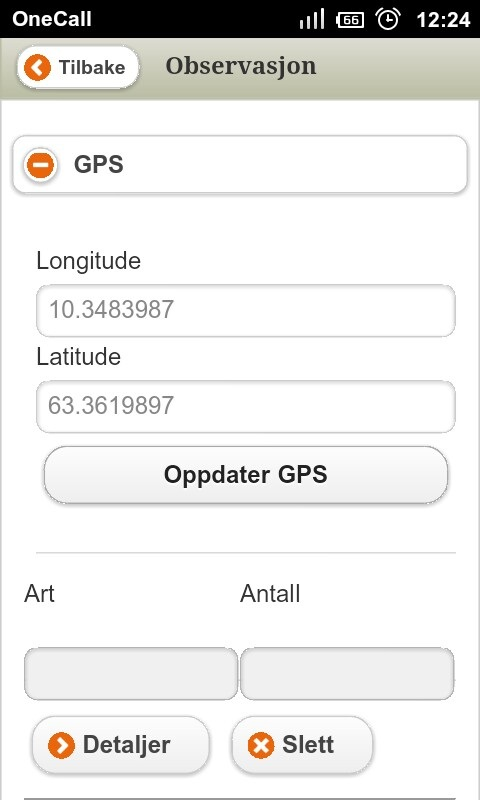
\includegraphics[height=0.7\textwidth]{appendix/pic/gps.jpg} 
 \caption{Gather location from GPS}
 \end{figure}

\pagebreak

\subsubsection{Add additional information}
From the observation page, the user can choose to add more information about the species observation by selecting "Add more information/Detaljer".

All fields are available for editing. Special input boxes for time and date
selection will open if date or time fields are edited.

\begin{figure}[h!]
\centering
 \begin{center}$
 \begin{array}{cc}
 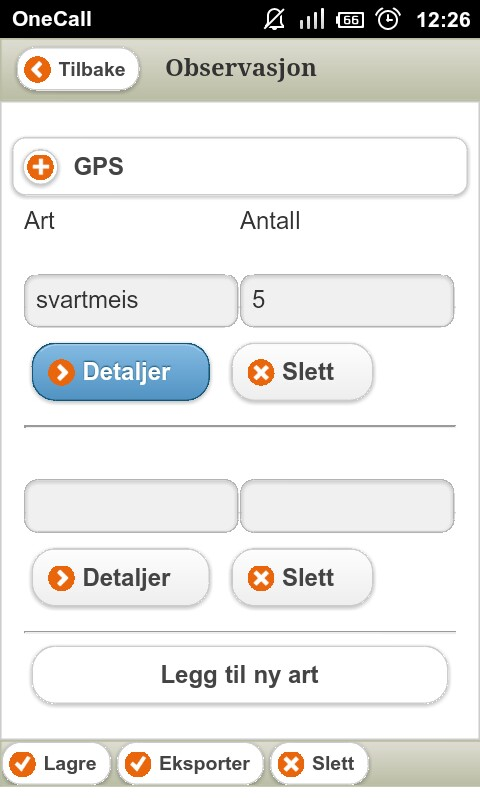
\includegraphics[width=0.45\textwidth]{appendix/pic/det1.jpg} &
 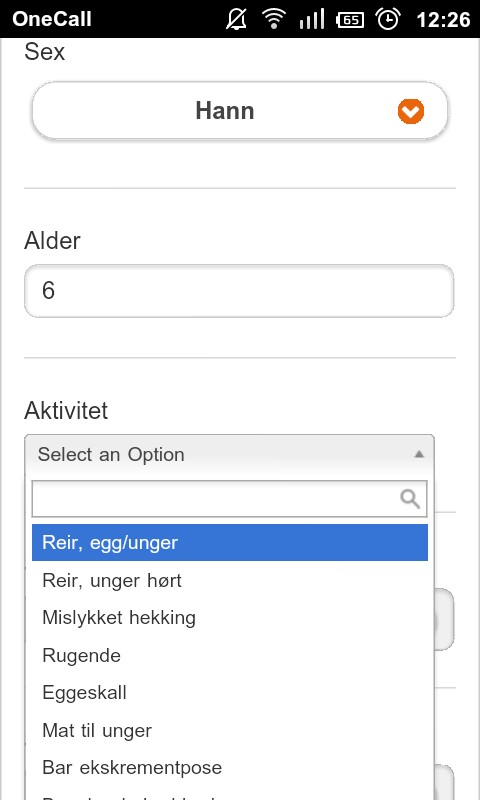
\includegraphics[width=0.45\textwidth]{appendix/pic/det2.jpg}
 \end{array}$
 \end{center}
 \caption{Observation page (left). Details page (right) }
 \end{figure}


\pagebreak


\subsubsection{Add pictures of a species}
At the bottom of the Extended information page the user may also include images from disk or camera, if the user clicks on an already existing image he/she can remove the picture from the observation again. The added picture will be displayed in the window.

\begin{figure}[h!]
\centering
 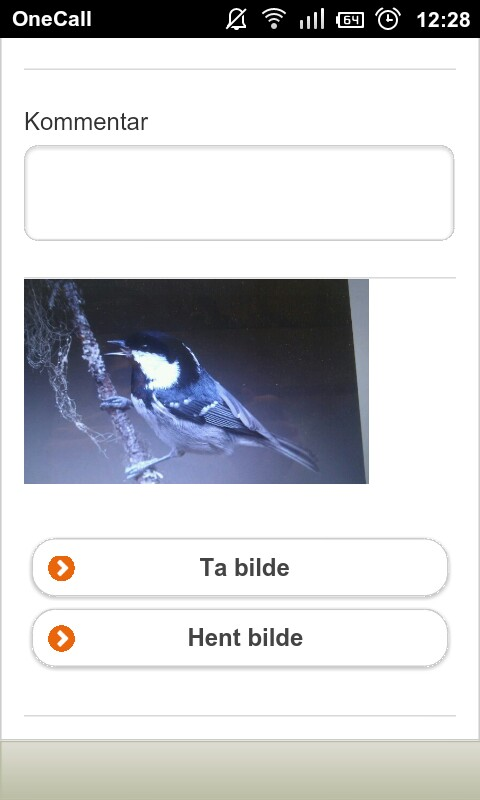
\includegraphics[height=0.9\textwidth]{appendix/pic/bilde.jpg} 
 \caption{Add pictures of a species}
 \end{figure}

\pagebreak

\subsubsection{Adding additional species to an observation}
The user may also add additional species to an observation via the "Add additional species/Legg til ny art" button in the  observation window. This will create a new row for that species.

\begin{figure}[h!]
\centering
 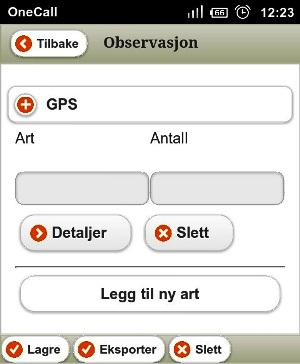
\includegraphics[height=0.6\textwidth]{appendix/pic/nyart.jpg} 
 \caption{Adding additional species to an observatio}
 \end{figure}

\subsubsection{Storing an observation}
To store an observation simply click the "Save/Lagre" button at the bottom of the observation.


\pagebreak

\subsubsection{Editing a stored observation}
To edit an existing observation the user can select "Saved observations/Lagrede Observasjoner" from the front page. 
This will list all saved observations on the device. 
These observations are identifiable from it's species type, date of creation and an id assigned to it.

\begin{figure}[h!]
\centering
 \begin{center}$
 \begin{array}{cc}
 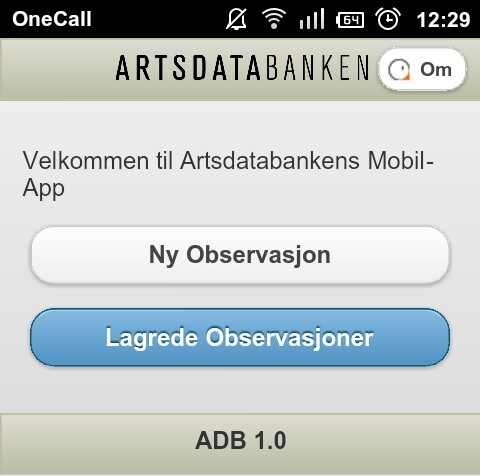
\includegraphics[width=0.45\textwidth]{appendix/pic/lagr1.jpg} &
 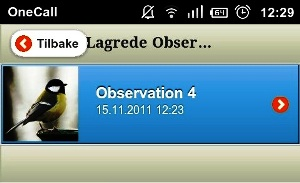
\includegraphics[width=0.45\textwidth]{appendix/pic/lagr2.jpg}
 \end{array}$
 \end{center}
 \caption{Front page (left). Stored Observations (right) }
 \end{figure}



\subsubsection{Exporting an observation}
To export an observation the user can click on the "Export/Eksporter" button at the bottom of the observation page.
This will open up a menu to select which application to use for exporting. THe
recommended choice is the GMail application.

The user is free to send the observation to any email address, and the received
email can be used on the web-page of Artsdatabanken by copying the entire email
body and pasting it in the import from XSL section.
Any images linked to the observation will be attached to the email.

\subsubsection{Deleting an observation}
An observation can be deleted by clicking the "Delete/Slett" button at bottom of an observation.
